\documentclass[10pt]{article}

\usepackage{amsmath}
%
\usepackage{amssymb}
%
\usepackage{enumerate}
%
\usepackage[width=7in,height=10in,top=0.75in,centering]{geometry}
%
\usepackage[dvipsnames]{xcolor}
%
\usepackage{tikz}
%
\usepackage{multicol}
%
\usepackage{hyperref}
%
\usepackage{marginnote}
%
\usepackage{pdfpages}
%
%%%%%%%%%%%%%%%% HEADER %%%%%%%%%%%%%%%%%%%%%
\usepackage{fancyhdr}
\pagestyle{fancy}
%%
%\lfoot{Left footer}
%\cfoot{Center of footer}
%\rfoot{Right of footer}
%%
\lhead{Survey of Calculus I}
\chead{Local Extrema \& the First Derivative Test}
\rhead{\thepage}
%
%%%%%%%%%%%%%%%% HEADER %%%%%%%%%%%%%%%%%%%%%
%
%%%%%%%%%%%%%%%% PGFPLOTS %%%%%%%%%%%%%%%%%%%
\usepackage{pgfplots}
%
\pgfplotsset{every axis/.append style={
                    axis x line=middle,    % put the x axis in the middle
                    axis y line=middle,    % put the y axis in the middle
                    axis line style={<->,color=black}, % arrows on the axis
                    %xlabel={$x$},          % default put x on x-axis
                    ylabel={$y$},          % default put y on y-axis
            }}
%
 \pgfplotsset{compat=1.14}
%
 \usepgfplotslibrary{fillbetween}
%%%%%%%%%%%%%%%% PGFPLOTS %%%%%%%%%%%%%%%%%%%
%
\parindent0pt
\fboxsep=0.25cm
%
\newcommand{\Heading}[2]{\fbox{{\Large\textbf{#1}}}\hfill\fbox{\textbf{#2}}\par\vspace{0.1in}}
%
\newcommand{\Name}[1]{\textbf{Name}:\quad#1\hrulefill}
%
\newcommand{\Target}[1]{\textbf{Learning Target(s):}\quad\fbox{#1}\par\medskip}
%
\DeclareMathOperator{\arcsec}{arcsec}
\DeclareMathOperator{\arccot}{arccot}
\DeclareMathOperator{\arccsc}{arccsc}
%
\newcounter{example}[section]
\newcounter{exercise}[section]
%
\newcommand{\important}[2]{\begin{center}\fbox{\begin{minipage}{.97\textwidth}\noindent\textbf{#1}\par#2\end{minipage}}\end{center}}
%
\newcommand{\defn}[1]{\begin{center}\fbox{\begin{minipage}{.97\textwidth}\reversemarginpar\marginnote{\textbf{Definition}}#1\end{minipage}}\end{center}}
%
\newcommand{\example}{\vspace{0.1in}{\textcolor{blue}{\textbf{Example \stepcounter{example}\theexample.}}}\hspace{0.1in}}
%
\newcommand{\exercise}{\vspace{0.1in}{\textcolor{blue}{\textbf{Exercise \stepcounter{exercise}\Alph{exercise}.}}}\hspace{0.1in}}
%
\newcommand{\answer}[0]{\reversemarginpar\marginnote{\rule[-8pt]{0.5in}{0.4pt}}}
%
\newcommand{\lt}[1]{\reversemarginpar\marginnote{\fbox{\bf #1}}}

%%%%%%%%%%%% BEGIN DOCUMENT %%%%%%%%%%%%%%%
%%%%%%%%%%%% BEGIN DOCUMENT %%%%%%%%%%%%%%%
%%%%%%%%%%%% BEGIN DOCUMENT %%%%%%%%%%%%%%%
%%%%%%%%%%%% BEGIN DOCUMENT %%%%%%%%%%%%%%%
%%%%%%%%%%%% BEGIN DOCUMENT %%%%%%%%%%%%%%%

%%%%%%%%%%%% BEGIN DOCUMENT %%%%%%%%%%%%%%%
%%%%%%%%%%%% BEGIN DOCUMENT %%%%%%%%%%%%%%%
%%%%%%%%%%%% BEGIN DOCUMENT %%%%%%%%%%%%%%%
%%%%%%%%%%%% BEGIN DOCUMENT %%%%%%%%%%%%%%%
%%%%%%%%%%%% BEGIN DOCUMENT %%%%%%%%%%%%%%%

\begin{document}

\thispagestyle{empty}

\Heading{MATH 1190 \& 1210 Survey of Calculus I}{\begin{minipage}{0.275\textwidth}\begin{center} Lesson 11:\\ Local Extrema \& the 1st Derivative Test \end{center}\end{minipage}}

\vspace{0.1in}

\Name{} \quad \Target{{\bf\color{RedOrange}A1}, {\bf\color{RedOrange}A2}}

\hrulefill\\

\paragraph*{Lesson Goals} related to targets {\bf\color{RedOrange} A1: Derivatives \& Graphing} \& {\bf\color{RedOrange} A2: Local \& Absolute Extrema}
\begin{itemize}
    \item Identify increasing/decreasing intervals and critical numbers of a function from given graph or formula. 
    \item Represent concepts such as derivatives, local extrema, and critical number graphically.
    \item Apply the First Derivative Test to determine the local extrema of a function graphically and algebraically.
\end{itemize}

{\it Feedback from Pre-class Activity} 

\begin{itemize}
\item Critical Points are still kind of confusing to me hoping to learn more in class!
\item I didn't understand why 0 and 2 weren't considered critical points even though they were where the function's derivative DNE.
    \begin{itemize}
    \item {\it DJ's note:} In the pre-class assignment, students are asked to identify critical numbers of $f(x)=\ln(2x-x^2)$, whose derivative is $f'(x)=\frac{2-2x}{2x-x^2}$. $f'$ DNE at $x=0$ \& $x=2$, but $f$ is not defined at either of these values. So, they cannot be critical numbers.
    \end{itemize}
\item The most interesting thing I found was Fermat"s theorem. Once I learned a little about it, I was able to find the critical points of some basic functions
\item {\it DJ's note:} Some additional slides involving the First Derivative Test were added during the Spring 2025 semester. Students will likely also have questions about using the First Derivative Test.
\end{itemize}

{\it Handout structure:}
\begin{itemize}
\item The first page of the lesson is part of a written pre-class assignment.
    \begin{itemize}
    \item {\bf\color{blue}Warm-up exercise 1} asks students to fill in 3 key parts of the definition of a critical number, and then gives them a chance to demonstrate understanding of those 3 key parts in asking whether $f(x)=\frac1x$ has exactly 1 critical number (it doesn't, as $f'$ is never 0 and $f$ is not defined where $f'$ DNE).
    \item {\bf\color{blue}Warm-up exercise 2} asks students to fill in blanks from the First Derivative Test seen in the pre-class activity, then {\bf\color{blue} warm-up exercise 3} gives students a chance to demonstrate understanding of the statement of that test. Students will need to know what it means graphically for $f'$ to be $+$, $-$, $0$, or $DNE$, activating prior knowledge of target {\bf\color{ForestGreen} D1}.
    \end{itemize}
You might put students in groups, assign each group 1 of the 3 exercises on page 1, give them 3 minutes to discuss, and then ask a group for each exercise to present their results. This helps keep the ownership of learning with the students. However, if you are behind, then you might fill in parts of page 1 to save time.
\item {\bf\color{blue}Example 1} is an immediate application of the concepts from page 1: critical numbers, knowing how the sign of the first derivative relates to whether the function $g(x)=x-\ln(x^2+1)$ is increasing/decreasing, and identifying local extrema using the First Derivative Test.
    \begin{itemize}
    \item The function was chosen deliberately so that two common issues can be addressed in part (a). The first issue is the misconception $\frac{d}{dx}[\ln(f(x))]$ always equals $\frac{1}{f(x)}$. The second issue is solving equations involving fractions - in this example, solving $g'(x)=0$ $\implies$ $1-\frac{2x}{x^2+1}=0$, and knowing that $g'(x)$ DNE when the denominator is made to be $0$. The latter doesn't occur in this example, but this should be shown explicitly so students know to check.
    \item In part (b), we'll find that $g'$ is only ever $+$ or $0$, indicating $g$ is only ever increasing or temporarily not. Still, it should be emphasized that $g'<0 \,\implies\, g$ is decreasing so students are ready for {\bf\color{blue}Exercise A}. Be sure to draw a sign line to summarize your results so students are ready to draw one in {\bf\color{blue} Exercise A}.
    \item In part (c), we need to model how students should write their answers. Stating the conclusion by directly invoking the statement of the First Derivative Test helps model how conclusions in mathematics are directly connected to established facts, so you might say something like ``$g'$ does not change signs at the critical number $x=1$, so $g$ has neither a local maximum nor local minimum there by the First Derivative Test."
    \end{itemize} 
\item {\bf\color{blue} Exercise A} repeats the skill we established in {\bf\color{blue}Example 1}. Importantly, the function in this exercise does have both a local maximum and local minimum, so you might be ready to support students in coming those conclusions using the First Derivative Test. Although students will have seen such an example in the pre-class assignment, they will still likely need some support here in showing their work. Leaving your work on {\bf\color{blue}Example 1} or the statement of the First Derivative Test on the board/projector screen will help scaffold the exercise.
\item {\bf\color{blue} Exercises B and C} gives students practice with the definition of a critical number and how a function relates to its first derivative, but graphically instead of algebraically. Students should be ready to flexibly and fluently move between algebraic and graphical representations of these concepts, so emphasizing the importance of the argument over the answer is critically important in this exercise.
\item {\bf\color{blue} Extra Practice 1} reviews the definition of a critical number. Students tend to bring in the misconception that a critical number can arise only from a zero derivative; this exercise helps them to see critical numbers can occur where the derivative DNE.
\item {\bf\color{blue} Extra Practice 2 \& 3} are repeats of {\bf\color{blue}Example 1} and {\bf\color{blue}Exercise A}.
\end{itemize}

%%%%%%%%%
\newpage%
%%%%%%%%%

\pagestyle{otherpages}
\thispagestyle{firstpage}
\vs{.6}

\textbf{Intended Learning Outcomes}
After this lesson, you will be able to 

\begin{itemize}
    \item Identify increasing/decreasing intervals and critical numbers of a function from given graph or formula. (\target{A1})
    \item Sketch graphs with given conditions involving derivatives, local extrema, and critical number. (\target{A1})
    \item Determine intervals for which a given function is increasing/decreasing algebraically. (\target{A1})
    \item Apply the first derivative to determine the local extrema of a function graphically and algebraically. (\target{A2})
\end{itemize}

\vspace{-0.5cm}

\hrulefill\\

In this activity, we establish a means of finding local extreme values (also called relative extreme values) of a function using properties of the derivative. First, review some key ideas from the online pre-class activity to prepare yourself for the important ideas of the lesson.\\

{\bf \textcolor{blue}{Warm-up exercise 1.}}  Fill in the blanks to complete the definition of a critical number, then respond to the prompt below.
%
 \important{Definition: Critical Number}
    {
    A {\bf critical number} of a function $f$ is a number $c$ at which $f$ is \blue{defined} and either
    \begin{center}
    $f'(c) = \blue{0}$ \quad\quad\quad or \quad\quad\quad $f'(c)$ \blue{DNE}.
    \end{center}
    }
    
    {\bf TRUE or FALSE?} $\displaystyle f(x)=\frac1x$ has exactly 1 critical number. \hfill (circle one): \hfill {\bf TRUE} \hfill {\bf FALSE}

    \blue{False. $f'(x)=-x^{-2}=-\dfrac{1}{x^2}$, so $f'(x)=0$ has no solution and $f'(x)$ DNE when $x=0$. However $f(0)$ is not defined, so $x=0$ is not a critical number of $f(x)$.}

{\bf \textcolor{blue}{Warm-up exercise 2.}} Fill in the blanks to complete the statement of the First Derivative Test as it appeared in the online pre-class activity.

\begin{minipage}[t][2.75in][t]{0.65\textwidth}
 \important{First Derivative Test}
{
Suppose that $c$ is a \blue{critical number} of a continuous function $f$.
\begin{enumerate}[(a)]
\item If $f'$ changes from \blue{positive} to \blue{negative} at $c$, then $f$ has a local maximum at $c$.
\item If $f'$ changes from \blue{negative} to \blue{positive} at $c$, then $f$ has a local minimum at $c$.
\item If $f'$ does not change sign at $c$, then $f$ has \blue{neither a local maximum nor a local minimum} at $c$.
\end{enumerate}
}
\end{minipage}
%
\hfill
%
\begin{minipage}[t][2.75in][t]{0.33\textwidth}
\,\\[-0.1in]

\includegraphics[width=0.95\textwidth]{images/1st derivative test.PNG}
\end{minipage}

\
 
\begin{minipage}[t]{0.6\textwidth}
{\bf \textcolor{blue}{Warm-up}}\exercise{\color{RedOrange}A1} Sketch the graph of a function $f$ satisfying the following:\\
 \begin{itemize}
 \item $f'(2)=0$ and $f(2)$ is a local/relative minimum
 \item $f'(4)=0$ and $f(4)$ is neither a maximum nor a minimum
 \item $f'(6)$ DNE and $f(6)$ is a local/relative maximum
 \end{itemize}
 \end{minipage}
 \hfill
 \begin{minipage}[t]{0.38\textwidth}
 \vspace{-0.2in}
 \begin{center}
	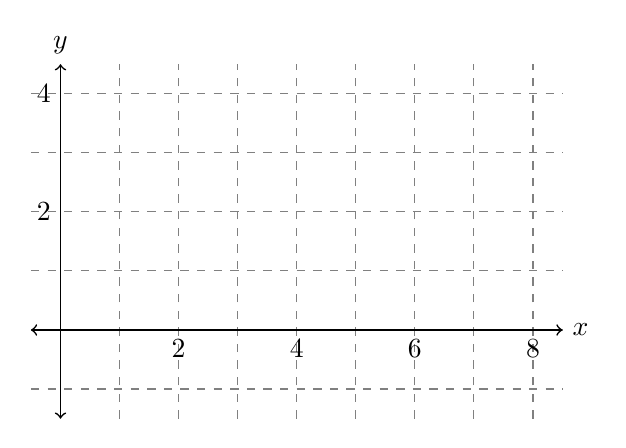
\begin{tikzpicture}[yscale=0.75,xscale=0.75]
	\draw[thin,color=gray,step=1,dashed] (-0.5,-1.5) grid (8.5,4.5); 
	\draw[semithick, <->] (-0.5,0)--(8.5,0) node[right]{$x$};   % x-axis
	\draw[semithick, <->] (0,-1.5)--(0,4.5) node[above]{$y$}; % y-axis
	\draw (2,0) node[below]{$2$};
	\draw (4,0) node[below]{$4$};
	\draw (6,0) node[below]{$6$};
	\draw (8,0) node[below]{$8$};
	\draw (0,2) node[left]{$2$};
	\draw (0,4) node[left]{$4$};
	\end{tikzpicture}
 \end{center}
 \end{minipage}

 %\end{document} %end here for written pre-class

 %%%%%%%%%%%%%
	%\newpage%%
 %%%%%%%%%%%%%

{\example{\color{RedOrange}A1,A2}} Let $g(x)=x-\ln(x^2+1)$.
%
\begin{enumerate}[(a)]
\item Find the critical numbers of $g$.

\blue{$g'(x)=1-\dfrac{1}{x^2+1}\cdot 2x=1-\dfrac{2x}{x^2+1}=\dfrac{x^2-2x+1}{x^2+1}=\dfrac{(x-1)^2}{x^2+1}$

If $g'(x)=0$, we get $(x-1)^2=1$, or $x=1$.

If $g'(x)$ DNE, we get $x^2+1=0$, which has no solution.

$g(1)=1-\ln(2)$ is defined. So $x=1$ is a critical number of $g(x)$.}

\item Find the intervals where $g$ is increasing or decreasing.

\blue{We can make a sign line to record the sign of $g'(x)$. The critical number $x=1$ splits the number line into two intervals. For each interval, we can plug in a value to determine the sign of $g'(x)$ on this interval.

$g'(0)=1-0=1>0$

$g'(2)=1-\dfrac{2\cdot 2}{2^2+1}=\dfrac{1}{5}>0$

\begin{center}
\begin{tikzpicture}[scale=1]
              \begin{axis}[
              axis y line=left,
            xlabel={$x$},
            ylabel={},
            xlabel style={anchor=west},
	  y axis line style={draw=none},
	  	  x axis line style={draw opacity=0},
            %grid = major,
            every major tick/.append style={ thick, blue, major tick length=5pt},
            xtick       = {  1},
            xticklabels = { $1$ },
            ytick       = \empty,
            yticklabels={},
                                      y  axis line style=-,
                          % y axis/.append style={y axis line style=-}
            samples     = 320,
            restrict y to domain=-40:40,
            xmin = -2, xmax = 3,
            ymin = -.5, ymax = 1.5,
            height=1.5in, width=2.75in
          ]
	\draw[thick,<->] (-1,0) -- (3,0);
	 \node[anchor=west] at (-1.5,.5) {\small $g^{\prime}(x)$};
	  	   \node at (1,.5) {\small $0$};
	    %\node at (-.8,.5) {\small $0$};
		\node at (0,.5) {\small $(+)$};
		\node at (2,.5) {\small $(+)$};
		%\draw[ultra thick, red] (-.8,1.5) -- (-.05,.8);
		%\draw[ultra thick, red] (.05,.8) -- (.8,1.5);
          %
        \end{axis}
    \end{tikzpicture}
\end{center}

Since $g'(x)$ is positive on the intervals $(-\infty, 1)$ and $(1, \infty)$, we get $g(x)$ is increasing on the intervals $(-\infty, 1)$ and $(1, \infty)$. $g(x)$ is never decreasing.

Note: We can't say $g(x)$ is increasing on $(-\infty, \infty)$ because $g(x)$ is not increasing at $x=1$.
}

\item At which critical number(s) does $g$ attain a local extreme value(s)? Explicitly cite a relevant test in your response.

\blue{The sign of $g'(x)$ does not change at its critical number $x=1$, so by the First Derivative Test, $g(x)$ has neither a local maximum nor a local minimum at $x=1$.}

\end{enumerate}

\newpage

{\exercise{\color{RedOrange}A1,A2}} Let $f(x)=\dfrac{x}{x^2+1}$.
\begin{enumerate}
\item[(a)]Find the intervals where $f$ is increasing or decreasing. Draw a sign line to depict your answer, and record your final answer using interval notation. \\

\blue{$f'(x)=\dfrac{(x^2+1)-x(2x)}{(x^2+1)^2}=\dfrac{1-x^2}{(x^2+1)^2}$

If $f'(x)=0$, we get $1-x^2=0$, or $x=\pm 1$.

If $f'(x)$ DNE, we get $(x^2+1)^2=0$, which has no solution.

Both $f(-1)=\dfrac{-1}{1+1}=-\dfrac{1}{2}$ and $f(1)=\dfrac{1}{1+1}=\dfrac{1}{2}$ are defined, so both $x=-1$ and $x=1$ are critical numbers of $f(x)$.

These two critical numbers split the number line into three parts. For each part, we plug in a number to determine the sign of $f'(x)$ on it.

$f'(-2)=\dfrac{1-4}{4+1}=-\dfrac{3}{5}<0$

$f'(0)=\dfrac{1-0}{0+1}=1>0$

$f'(2)=\dfrac{1-4}{4+1}=-\dfrac{3}{5}<0$

\begin{center}
\begin{tikzpicture}[scale=1]
              \begin{axis}[
              axis y line=left,
            xlabel={$x$},
            ylabel={},
            xlabel style={anchor=west},
	  y axis line style={draw=none},
	  	  x axis line style={draw opacity=0},
            %grid = major,
            every major tick/.append style={ thick, blue, major tick length=5pt},
            xtick       = { -1, 1},
            xticklabels = { $-1$, $1$ },
            ytick       = \empty,
            yticklabels={},
                                      y  axis line style=-,
                          % y axis/.append style={y axis line style=-}
            samples     = 320,
            restrict y to domain=-40:40,
            xmin = -4, xmax = 3,
            ymin = -.5, ymax = 1.5,
            height=1.5in, width=2.75in
          ]
	\draw[thick,<->] (-3,0) -- (3,0);
	 \node[anchor=west] at (-4,.5) {\small $f^{\prime}(x)$};
	  	\node at (1,.5) {\small $0$};
	    \node at (-1,.5) {\small $0$};
		\node at (0,.5) {\small $(+)$};
        \node at (-2,.5) {\small $(-)$};
		\node at (2,.5) {\small $(-)$};
		%\draw[ultra thick, red] (-.8,1.5) -- (-.05,.8);
		%\draw[ultra thick, red] (.05,.8) -- (.8,1.5);
          %
        \end{axis}
    \end{tikzpicture}
\end{center}

Therefore, $f(x)$ is increasing on the interval $(-1, 1)$, and $f(x)$ is decreasing on the intervals $(-\infty, -1)$ and $(1, \infty)$.

}

\vfill

\item[(b)]Find the local maximum \& local minimum points of $f$. Explicitly cite a relevant test in your response. \\

\blue{$f'(x)$ changes from negative to positive at $x=-1$, so by the First Derivative Test, $f(x)$ has a local minimum at $x=-1$.

$f'(x)$ changes from positive to negative at $x=1$, so by the First Derivative Test, $f(x)$ has a local maximum at $x=1$.}

\vfill

\end{enumerate}

\newpage

\paragraph*{Note:} The next problem will test your conceptual understanding of what it means for a function to increase or decrease, as well as of the definition of a critical number. A variation of this problem appeared on an exam during the Fall 2023 semester.\\

\begin{minipage}{0.55\textwidth}
\exercise{\color{RedOrange}A1}  What would the critical numbers of the function $f$ be if...
\begin{enumerate}
\item[(a)] the curve pictured to the right is the graph of $f$?
\item[(b)] the curve pictured to the right is the graph of $f'$?
\end{enumerate}
On which intervals would the function $f$ be {\it decreasing} if...
\begin{enumerate}
\item[(c)] the curve pictured to the right is the graph of $f$?
\item[(d)] the curve pictured to the right is the graph of $f'$?
\end{enumerate}
\end{minipage}
%
\begin{minipage}{0.45\textwidth}
\begin{center}
    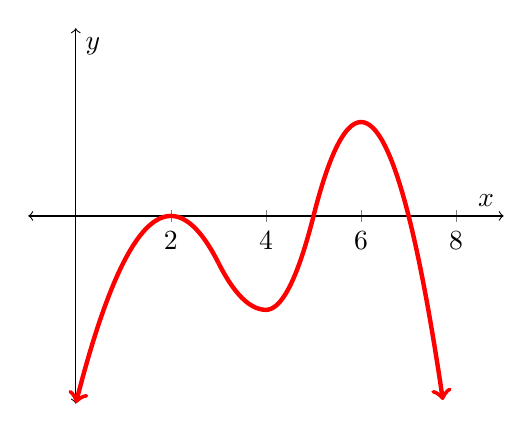
\begin{tikzpicture}[scale=1]
          \begin{axis}[
            xlabel={$x$},
            %grid = major,
            xtick       = {2,4,6,8},
            xticklabels = {$2$,$4$,$6$,$8$},
            ytick       = {0},
            yticklabels = {$0$},
            samples     = 320,
            domain      = -1:9,
            restrict y to domain=-4:4,
            xmin = -1, xmax = 9,
            ymin = -4, ymax = 4,
            height=2.5in, width=3in
          ]
          % old version of the curve
          %
          %\addplot[domain=-1:9, purple, ultra thick, mark=none] {-1/10*(x-1)*(x-4)^2*(x-7)};
          %
          %new version of the curve in pieces
          %
          \addplot[domain=-1:3, ultra thick, red,<-] {-(x-2)^2};
          \addplot[domain=3:4, ultra thick, red] {(x-4)^2-2};
          \addplot[domain=4:5, ultra thick, red] {2*(x-4)^2-2};
          \addplot[domain=5:9, ultra thick, red,->] {-2*(x-6)^2+2};
          %
        \end{axis}
    \end{tikzpicture}
\end{center}
\end{minipage}\\

\vspace{0.1in}

\,\hfill
\fbox{
    \begin{minipage}{ 0.18\textwidth}
    {\bf ANSWER (a):}
        \blue{$x=2, 4, 6$}
    \end{minipage}
    }
\hfill
    \fbox{
    \begin{minipage}{ 0.18\textwidth}
    {\bf ANSWER (b):}
        \blue{$x=2, 5, 7$}
    \end{minipage}
    }
\hfill
\fbox{
    \begin{minipage}{ 0.18\textwidth}
    {\bf ANSWER (c):}
        \blue{$(2, 4)$ and $(6, \infty)$}
    \end{minipage}
    }
\hfill
    \fbox{
    \begin{minipage}{ 0.18\textwidth}
    {\bf ANSWER (d):}
        \blue{$(-\infty, 2)$, $(2, 5)$, and $(7, \infty)$}
    \end{minipage}
    }
\hfill\,\\

Space is provided below for you to explain your answers.

\blue{(a) Suppose the given graph is of $f$. We can see that $f$ has horizontal tangent lines at $x=2, 4, 6$, which means $f'(x)=0$ at them. $f$ is clearly defined at these three points, so these three points are critical numbers of $f$. In addition, $f$ is a smooth curve with no corners, vertical tangents, nor discontinuities, so $f$ has no additional critical numbers.

(b) Suppose the given graph is $f'$. The graph has a $y-$value of $0$ at $x= 2, 5, 7$, so these are the points where $f'(x)=0$, which means they are critical numbers of $f$. Since $f'$ is defined everywhere in the graph, $f$ has no additional critical numbers.

(c) Suppose the given graph is of $f$. Then $f$ is decreasing on $(2, 4)$ and $(6, \infty)$.

(d) Suppose the given graph is $f'$. The $y$-value is negative on the intervals $(-\infty, 2)$, $(2, 5)$, and $(7, \infty)$, so $f$ is decreasing on these intervals.}

\vfill

\paragraph*{Note:} The next problem will test your comprehension of warm-up exercise 1 and the Chain Rule.\\

{\bf\color{blue} Extra Practice 1.} \reversemarginpar\marginnote{\fbox{\bf\color{RedOrange} A2}} Find all critical numbers of $f(x)=\sqrt[3]{x^2-4x}$.

\blue{
$f(x)=(x^2-4x)^{1/3}$

$f'(x)=\dfrac{1}{3}(x^2-4x)^{-2/3}(2x-4)=\dfrac{2x}{3(x^2-4x)^{2/3}}$

If $f'(x)=0$, we get $2x-4=0$, or $x=2$.

If $f'(x)$ DNE, we get $x^2-4x=0$, or $x(x-4)=0$. This gives $x=0$ and $x=4$.

The domain of $f$ is all real numbers, so $f$ is defined at $x=0, 2, 4$, which means these three numbers are the critical numbers of $f$.

}

\vfill

\newpage

\paragraph*{Note:} The next 2 exercises make use of all the information in this worksheet and the associated pre-class activity. The goal is for you to continue to fluently apply the definition of a critical number, to find \& interpret the sign of the first derivative as it relates to whether a function is increasing or decreasing, and to use the First Derivative Test to classify critical numbers.\\

{\bf\color{blue} Extra Practice 2.} \reversemarginpar\marginnote{\fbox{\bf\color{RedOrange} A1, A2}} Let $f(x)=\ln(x^2-2x+1)$. 
\begin{enumerate}[(a)]
\item Find all critical numbers of $f$.
    
\blue{
$f'(x)=\dfrac{2x-2}{x^2-2x+1}=\dfrac{2(x-1)}{(x-1)^2}=\dfrac{2}{x-1}$

If $f'(x)=0$, we get $2=0$, which is impossible.

If $f'(x)$ DNE, we get $x-1=0$, or $x=1$.

$f(1)=\ln(1-2+1)=\ln(0)$, which is undefined. So $f(x)$ has no critical number.

}
    
\vfill
    
\item Find the intervals on which $f$ is increasing \& the intervals on which $f$ is decreasing.

\blue{

Even if $x=1$ is not a critical number, it is a point where $f'(x)$ DNE, so we still use it to split the number line into two parts.

$f'(0)=\dfrac{2}{0-1}=-2<0$

$f'(2)=\dfrac{2}{2-1}=2>0$

\begin{center}
\begin{tikzpicture}[scale=1]
              \begin{axis}[
              axis y line=left,
            xlabel={$x$},
            ylabel={},
            xlabel style={anchor=west},
	  y axis line style={draw=none},
	  	  x axis line style={draw opacity=0},
            %grid = major,
            every major tick/.append style={ thick, blue, major tick length=5pt},
            xtick       = {  1},
            xticklabels = { $1$ },
            ytick       = \empty,
            yticklabels={},
                                      y  axis line style=-,
                          % y axis/.append style={y axis line style=-}
            samples     = 320,
            restrict y to domain=-40:40,
            xmin = -2, xmax = 3,
            ymin = -.5, ymax = 1.5,
            height=1.5in, width=2.75in
          ]
	\draw[thick,<->] (-1,0) -- (3,0);
	 \node[anchor=west] at (-1.5,.5) {\small $f^{\prime}(x)$};
	  	   \node at (1,.5) {\small $DNE$};
	    %\node at (-.8,.5) {\small $0$};
		\node at (0,.5) {\small $(-)$};
		\node at (2,.5) {\small $(+)$};
		%\draw[ultra thick, red] (-.8,1.5) -- (-.05,.8);
		%\draw[ultra thick, red] (.05,.8) -- (.8,1.5);
          %
        \end{axis}
    \end{tikzpicture}
\end{center}

Therefore, $f(x)$ is increasing on the interval $(1, \infty)$, and $f(x)$ is decreasing on the interval $(-\infty, 1)$.

}

    \vfill
    \vfill

\item At which $x$-values does $f$ have local maximum values? At which $x$-values does $f$ have local minimum values? Explain.

\blue{

$f$ has no local extrema since $f$ has no critical number.

}
    
    \vfill
\end{enumerate}

%%%%%%%%%
\newpage%
%%%%%%%%%

{\bf\color{blue} Extra Practice 3.} \reversemarginpar\marginnote{\fbox{\bf\color{RedOrange} A1, A2}}

Let $f(x)=\dfrac15x^5-\dfrac53x^3+4x$.
\begin{enumerate}[(a)]
\item Find the critical numbers of $f$.
    
\blue{

$f'(x)=x^4-5x^2+4=(x^2-4)(x^2-1)=(x-2)(x+2)(x-1)(x+1)$

If $f'(x)=0$, we get $x=-2, -1, 1, 2$.

There's no $x$-values for which $f'(x)$ DNE, since $f'(x)$ is a polynomial defined for all real numbers.

So the critical numbers of $f(x)$ are $x=-2, -1, 1, 2$.

}
    
    \vfill
\item Find the intervals where $f$ is increasing or decreasing.
    
\blue{

The critical numbers split the number line into five intervals: $(-\infty, -2)$, $(-2, -1)$, $(-1, 1)$, $(1, 2)$, and $(2, \infty)$.

\begin{table}[h!]
    \centering
    \begin{tabular}{c|cccc|c}
      $x$  & $x+2$ & $x+1$ & $x-1$ & $x-2$ & $f'(x)$\\
      \hline
        $(-\infty, -2)$ & - & - & - & - & +\\
        $(-2, -1)$ & + & - & - & - & -\\
        $(-1, 1)$ & + & + & - & - & +\\
        $(1, 2)$ & + & + & + & - & -\\
        $(2, \infty)$ & + & + & + & + & +\\
    \end{tabular}
\end{table}

Therefore, $f(x)$ is increasing on the intervals $(-\infty, -2)$, $(-1, 1)$, $(2, \infty)$, and $f(x)$ is decreasing on the intervals $(-2, -1)$ and $(1, 2)$.

}  
    
    \vfill
    \vfill
\item At which critical number(s) does $f$ attain local extrema? Explain.
    
\blue{

At $x=-2$ and $x=1$, $f'(x)$ changes from positive to negative, so by the First Derivative Test, $f$ has local maxima at these critical numbers.

At $x=-1$ and $x=2$, $f'(x)$ changes from negative to positive, so by the First Derivative Test, $f$ has local minima at these critical numbers.
}

    \vfill
    \vfill
\end{enumerate}

\end{document}